

\chapter{Conclusion}



\section{Same Sign}\label{sect:conclusion}

This section described a search for exotic processes in the same-sign dilepton plus jets signature with the ATLAS detector at LHC at $\sqrt{s}=7 \TeV$.
The searched used the full 2011 ATLAS $pp$ dataset, and selected events by requiring at least two jets, including at least one $b$-tagged jet, $\met>40 \GeV$ and $\HT>550 \GeV$, where \HT{} denotes the scalar sum of the \pT{} of all leptons and jets. 

Four events have been observed in this signal region with an expected background of $5.6\pm1.7$ events. 
This result has been interpreted in terms of several new physics models, including the pair production of down-type heavy quarks ($b^\prime$), the single and pair production of heavy quark partners ($T_{5/3}$), and the production of events containing four top quarks through a four-top quark contact interaction. 
The various limits which have been set are summarized in Table~\ref{limit:all}.



\begin{figure}[ht!]
  \begin{center}
    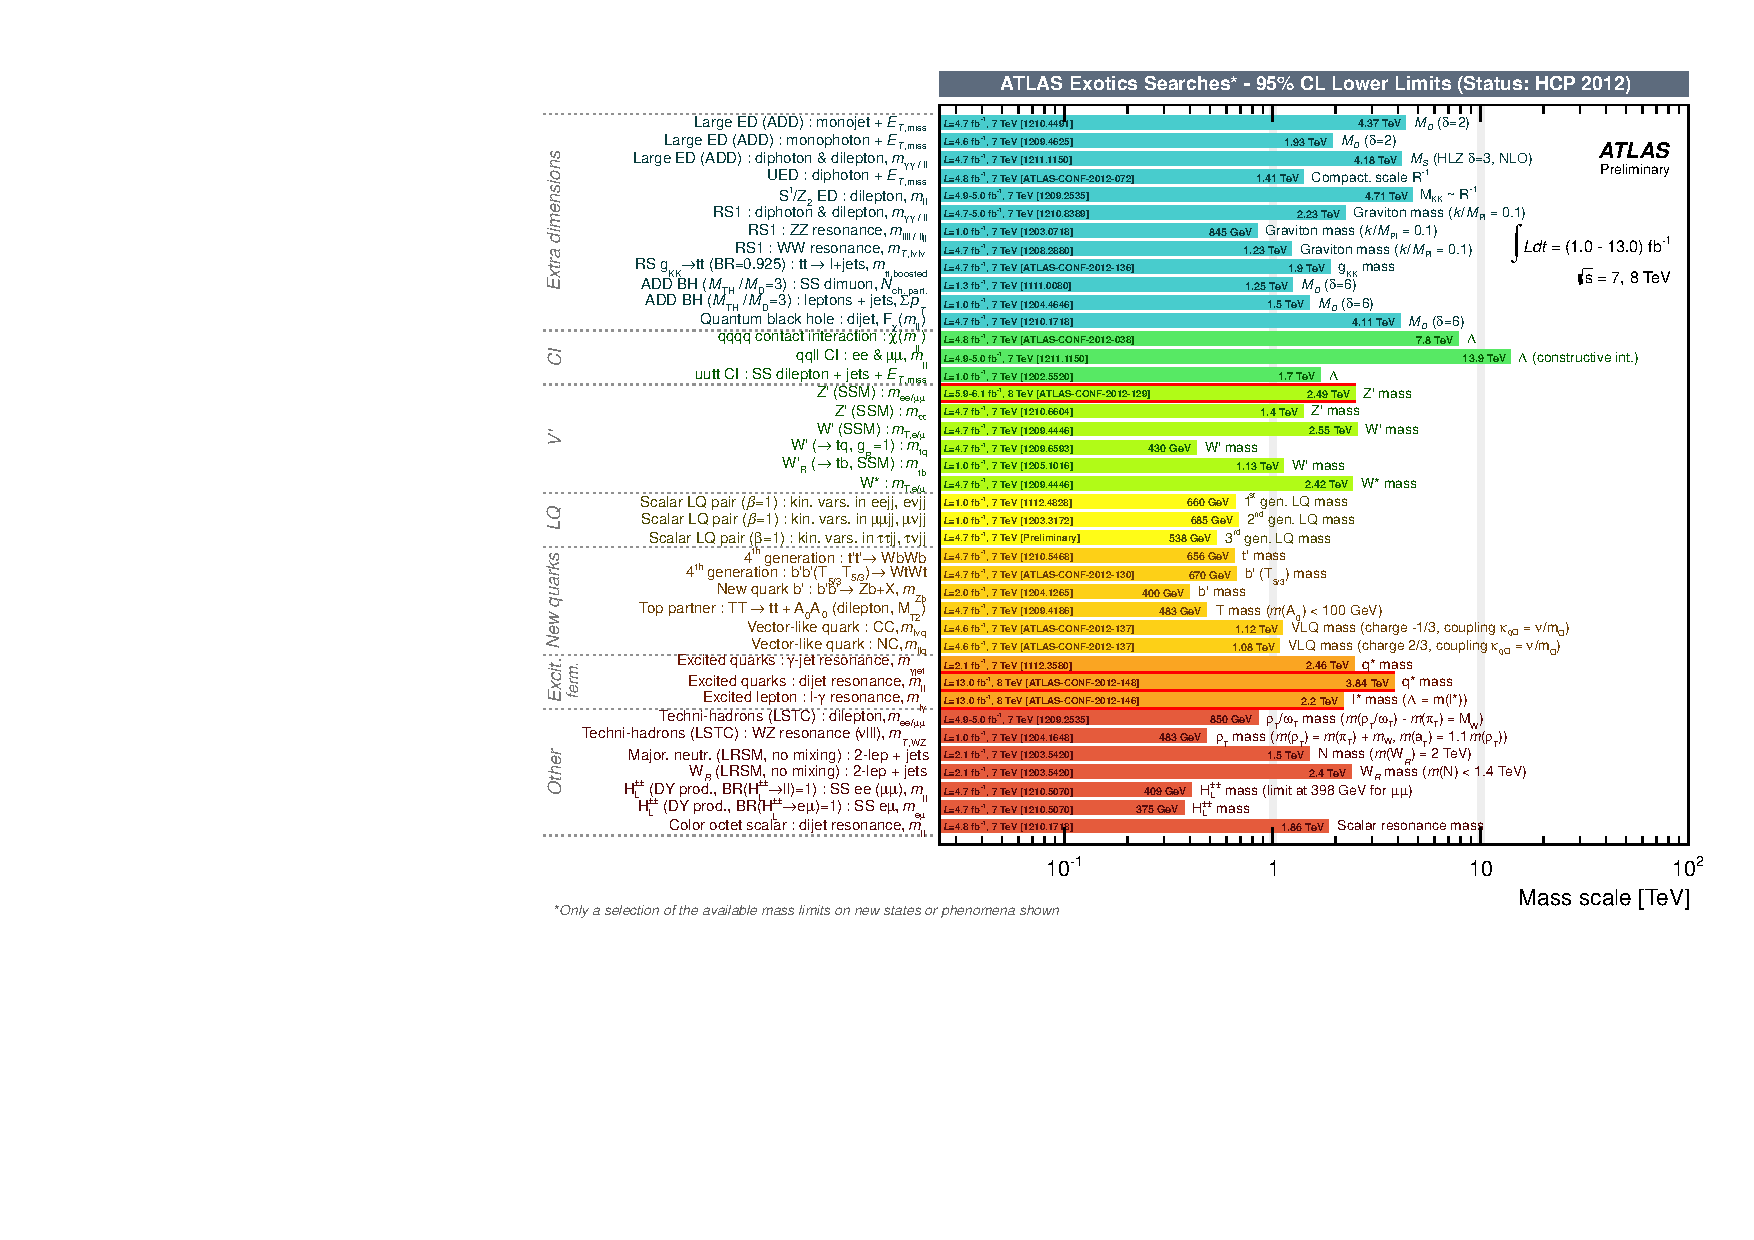
\includegraphics[width=.95\textwidth]{figures/conclusion/ExoticResultsSummary}
    \caption{Things}
    \label{fig:xsec_vs_roots}
  \end{center}
\end{figure}


